\section{Engineering traffic with location diversity}
\label{sec:locdiv-background}

In this section, we introduce location diversity, explain how it changes the traffic engineering problem, and introduce a new metric to quantify the capacity achieved by traffic engineering schemes with location diversity.

%\subsection{Traffic engineering}

%\subsubsection{TE Objectives}

%\textbf{TE objectives}

%ISP network operators use traffic engineering (TE) to achieve a variety of objectives that include minimizing congestion in the network, making long term network capacity provisioning decisions, ensuring quality-of-service for different classes of traffic, computing backup routes for link failures, and scheduling maintenance operations \cite{rexford,RFC3272}.   Our focus in this paper is on the goal of minimizing congestion based on intradomain traffic matrices, which has received the most amount of attention from researchers as well as network operators\tbd{All references here are to researchers. Do we have any references to support the network operators claim?} \cite{COPE1,TeXCP06,FortzThorup,ObliviousRouting,RFC3272,rexford}. 

%While other factors such as interdomain traffic and backup routes in network affect congestion as well, we exlcude them in this paper.

%\textbf{TE as optimization problem}

%Traditionally, the traffic engineering problem has been studied as an optimization problem that takes as input a traffic matrix and seeks to compute routes so as to minimize a network cost function. The cost function is intended to capture the severity of congestion hotpsots in the network based on link utilization levels. For example, the most widely used cost function, MLU, is simply the utilization of the most utilized link in the network \cite{COPE1,TeXCP06,MultiTM,ObliviousRouting}; another proposed by Fortz and Thorup \cite{FortzThorup,FortzThorup2} sums over all links a convex (so as to penalize highly utilized links more) function of their utilization levels. There are two implicit assumptions underlying this body of work. First, maintaining low link utilization levels improves user-perceived application performance under typical load conditions. Second, maintaining low link utilization levels increases the effective capacity of the network by enabling it to accommodate unexpected surges in the traffic demand.

%The problem of minimizing congestion has been widely studied till now as an optimization problem which minimizes a network cost function. The most widely used network cost function is maximum link utilization (MLU) \cite{COPE1,TeXCP06,MultiTM,ObliviousRouting}; other cost functions based on link utilization have also been considered \cite{FortzThorup,FortzThorup2}. There are two reasons for using link utlization based metrics : (1) A low utilization for all links implies that network is free of congestion (2) it implies such a network can accommodate a greater increase in traffic demand. This increase could be because of short term traffic spikes \cite{COPE1} or due to long term increase in overall network traffic.

%\subsubsection{Impact of TE on application performance}

%\textbf{TE metric does not measure app performance}

%Our work questions both of the above assumptions. The distinguishing aspect of our work is an application-centric approach to the traffic engineering problem: instead of posing TE as as optimization problem seeking to minimize link utilization, we focus on application performance metrics such as TCP throughput or delay for elastic  traffic and quality-of-service metrics (e.g., MOS metric for VoIP quality) for inelastic traffic. Accordingly, our evaluation methodology is empirical: instead of relying on mathematical simulations based on linear programming or heuristic techniques for NP-complete problems, our experiments carefully simulate end-to-end application behavior and compare different TE schemes with respect to their impact on application performance. 

%Our application-centric and empirical approach reveals rather unexpected results. We find that metrics based on link utilization alone, and in particular MLU, are a poor proxy for application performance. For example, a TE scheme may incur twice the MLU of another TE scheme and yet achieve as good or better application performance. The key reason for this mismatch is that application performance is largely determined by end-to-end loss rate and delay, but link utilization does not capture them accurately. At typical Internet loads, and in fact until the utilization starts approaching the capacity, link loss rates remain negligibly small. This observation has also been confirmed by explicit measurements on Internet backbones \cite{ExpRouterBuffer}, and is consistent with studies on the Sprint backbone \cite{Sprint} that show that over 90\% of all packet loss is caused by interdomain routing fluctuations as opposed to high utilization. Furthermore, end-to-end Internet path delays are largely determined by propagation delays as opposed to  queueing delays except at extremely high utilization.

%Although link utilization based metrics may seem reasonable to quantify the capacity of TE schemes, i.e., their ability to tolerate surges in traffic demand, we find that even this is not true in the light of application adaptation to location diversity, as we discuss in detail next.

%We claim that link utilization based cost functions are poor metrics to measure network wide application performance. Following reasons support our claim : (1) Loss rates and queuing delay on a link which affects application performance remain nearly zero until a very high value of link utilzation. Both measurements on internet backbone links \cite{ExpRouterBuffer} as well as our simulation of links upto few hundred Mbps verify this statement. (2) MLU is most widely used cost function but it may not reflect aggregate performance of the network. A high MLU could be due to higher utilization of one or a few links in the network while the rest of the links do not have any congestion.  (3) Link utilization based cost functions are further inadequate since they do not measure the delay in the network which is an important factor in application performance.

%\textbf{To meaure app performance, we need new metrics and a new simulation approach}

%A comparison of application performance for TE schemes needs new metrics as well as a new simulation approach. In constrast to prior research, which has mostly used link utilization based metrics, we select application performance metrics  for our study - (1) TCP throughput (2) VoIP call quality for UDP traffic.  Techniques to evaluate TE performance have relied on mathematical simulations, e.g., linear programs or heurisitic techniques for NP-complete problems, which compute link utilization values in the network. Clearly, link utilzation values are not enough to accurately measure end-to-end application performance. To this end, we build a simulation setup using ns-2 \cite{ns2} which simulates ISP traffic matrices  and measures TCP throughput and VoIP call quality metric. To our knowledge, this is the first comparison study of TE schemes using large scale packet level simulation of traffic matrices.

%TE is a involves multiple tasks (1) Network measurement to estimate performance and workload (2) modeling the network components and building simulation tools to analyze the network performance under different TE solutions (3) Optimizing network performance by computing solutions based on network models and measurements. ISPs configure intradomain and interdomain routing protocols based on solutions of TE problem to achieve desired objectives.


%Over the past decade considerable work has been done in the area of traffic engineering with the objective of finding traffic engineering methods, which optimize traffic using either OSPF or MPLS  \cite{MPLSIntro, FortzThorup}; optimize over multiple traffic matrices \cite{MultiTM}; or optimize for unpredictable traffic demands in the network. Traditionally, TE research has mainly focused on minimizing the congestion (by minimizing MLU \cite{COPE1,TeXCP06,MultiTM,ObliviousRouting}) in Network and, thereby, improving the network capacity.  There has been no significant work for studying the impact of TE on TCP/UDP application performance. Hence an important motivation behind our study is to find the effect (positive/negative) that current TE methods might have on end-to-end application performance. Surprisingly, as our results in section 4 shows, all TE schemes achieve nearly identical application performance. This reveals the failure of existing popular TE methods to capture/address aplication performance issues specifically.


%-	While cost functions based 

%Traffic engineering (TE) determines how to route traffic through a network to optimize a network-wide objective. Internet Service Providers (ISPs) use traffic engineering for a variety of objectives that include minimizing congestion hotspots, computing backup routes to accommodate links that fail or are taken down for maintenance, making longer term capacity provisioning decisions, optimizing interdomain transit cost or revenue, and so on \cite{rexford}.

%Our focus in this paper is first of these objectives, minimizing congestion, which has received the most amount of attention from researchers as well as network operators \cite{COPE1}, \cite{TeXCP06}, \cite{FortzThorup}, \cite{ObliviousRouting}. The most commonly used optimization objective for TE is to minimize the maximum link utilization (MLU) in the network \cite{COPE1,TeXCP06,MultiTM,ObliviousRouting}. Minimizing MLU has been the mantra of TE research and the minimum MLU TE scheme is considered the optimal scheme.  Other cost functions based on link utilization have also been considered where cost of a link is a convex function of link utilization and the aggregate cost of all links in the network is minimized \cite{MATE1,FortzThorup}.

%From an ISP's perspective minimizing the MLU reduces the load on the most congested link in the network. Implicitly, it is expected to improve application performance in the network. Another reason why the minimum MLU  TE scheme is prescribed for ISPs is to help the network cope with an increase in traffic demands. This increase could either be due to future increase in overall network traffic \cite{TeXCP06} or due to short-term unexpected spikes in traffic \cite{COPE1}. Minimizing MLU is believed to help the network cope with a greater demand and hence increases its capacity.


%\textbf{methods of TE}

%Over the past decade considerable work has been done in the area of traffic engineering with the objective of finding traffic engineering methods, which optimize traffic using either OSPF or MPLS  \cite{MPLSIntro, FortzThorup}; optimize over multiple traffic matrices \cite{MultiTM}; or optimize for unpredictable traffic demands in the network. Traditionally, TE research has mainly focused on minimizing the congestion (by minimizing MLU \cite{COPE1,TeXCP06,MultiTM,ObliviousRouting}) in Network and, thereby, improving the network capacity.  There has been no significant work for studying the impact of TE on TCP/UDP application performance. Hence an important motivation behind our study is to find the effect (positive/negative) that current TE methods might have on end-to-end application performance. Surprisingly, as our results in section 4 shows, all TE schemes achieve nearly identical application performance. This reveals the failure of existing popular TE methods to capture/address aplication performance issues specifically.




%\textbf{How do MLU-based traffic engineering schemes impact application performance?}

%We find that MLU and other link utilization based metrics are a poor predictor of network-wide application performance.  Higher link utilizations worsen application performance since they cause loss rate and queuing delay to increase. But, in our experiments we observe that both  loss rate and queuing delay do not increase perceptibly unless the link utilization is above a threshold value (0.6 in our experiments). Below this threshold link utilization makes little difference to application performance. Second, a high MLU does not mean a significant portion of network is congested. It could be due to higher utilization of one or a few links in the network while the rest of the network may be free from congestion. Third, the delay between source and destination is an important factor in application performance. Link utilization based metrics are further inadequate since they do not measure the delay in the network.



%We start with a simple observation that minimizing the MLU may not receive the best throughput in  a network. We take the example of a simple topology with two nodes A and B. There are three links between source node A and destination node B with the same capacity 1 Gbps but different link delays of 10 ms, 20ms and 30ms. The  average traffic between A and B is 200Mbps. The MLU would be minimized by splitting traffic equally among three paths, with an  average delay of 20ms. In contrast a shortest path routing scheme which sends all traffic on the 10ms delay link, would have half the average delay and it can possibly achieve faster download rates. 


%There exists signicant path diversity in ISP networks. Optimal scheme seeks to exploit this diversity but may increase delay. In contrast, even naive routing scheme such as shortest path routing with link weights inverse of capacity can give same or better throughput under network conditions with low loads.  Our objective is to empirically measure the application performance of different routing schemes on ISP topologies and real TMs under realistic access link bottlenecks.




%Traffic engineering (TE) is done by ISPs, the objective of traffic engineering is to make capacity and provisioning decisions and to avoid congestion in the network. The process of traffic engineering typically involves estimating the traffic demand, which is represented in terms of a traffic matrix, and computing a routing in the network based on a single or a set of traffic matrices.


%The cost function which is most widely considered is to minimize the maximum link utilization across all links in th enetwork (MLU) \cite{COPE1,TeXCP06,MultiTM,ObliviousRouting}. 

%The cost function widely used for traffic engineering is the maximum link utilization of an ISP network. 



\subsection{Location diversity: Prevalence}

%\subsection{Location Diversity in Internet}
%Location diversity and application adaptation due to it is widespread in Internet today.

%\subsubsection{Examples of location diversity}

Location diversity, or the ability to download content from multiple potential locations, is widespread in the Internet today. Major commercial CDNs, e.g., Akamai \cite{Akamai}, Level-3 \cite{Level-3}, EdgeCast \cite{edgecast} etc., commonly replicate content at hundreds of locations and redirect users to the best server based on proximity or dynamic monitoring of server and network congestion \cite{akamai-detour}. Popular P2P applications such as BitTorrent \cite{bittorrentprotocol}, PPLive \cite{PPLive} download content simultaneously from many peers that are chosen based on a number of factors including network congestion. Other examples of location diversity include cloud computing infrastructure providers such as Google and Amazon with geographically distributed sites; content hosting services such as Carpathia \cite{Carpathia}, Rapidshare \cite{OneClickHosting}, etc.; mirrored websites such as SourceForge, Debian, etc. 
% and in some cases based on 

%\noindent\textbf{CDNs:} 
%Major content distribution networks such as Akamai \cite{Akamai}, Level-3 \cite{Level-3}, EdgeCast \cite{EdgeCast} have servers at numerous locations in the internet and choose the best set of servers for each user depending on users location, server load as well as congestion in the network. Akamai for example adapts to congestion quickly and changes its set of servers within few seconds to few minutes \cite{akamai-detour}. 

%\noindent\textbf{P2P File Sharing:} Popular P2P file sharing applications such as BitTorrent \cite{BitTorrentRef} also leverage location diversity. A BitTorrent client downloads a file from multiple peers simultaneously which are likely in geographically diverse locations. A peer also keeps changing its set of peers it downloads from and continuously keeps choosing faster peers for download. This mechanism makes it tolerant to congestion in the network.

%\noindent\textbf{Cloud computing and content hosting services:} Major companies which provide services on using cloud computing infrastructure such as Google and Amazon have servers located at geographically distributed locations\cite{GoogleServerLocation}. The same is true for content hosting services such as Carpathia \cite{Carpathia} and Rapidshare \cite{OneClickHosting}. These infrastructures though are less reponsive to congestion in the network.

%\noindent\textbf{Mirroring}  is widely used technique in Internet by websites such as SourceForge and projects such as Debian and Ubuntu to provide location diversity benefits \cite{MirrorWiki}.

%Internet applications also use adaptation which exploits \emph{path diversity} using detour routing like techniques \cite{Detour}. Skype, the most popular VoIP and video calling application, connects users using multiple routes and dynamically chooses the one that is best suited at the time \cite{Skype}. CDNs also use detour routing for data transfer among their servers \cite{Akamai}.

%\subsubsection{Extent of Location Diversity}

% CDNs - cloud computing type traffic

Although quantifying the extent of location diversity in today's Internet is difficult, back-of-the-envelope calculations based on existing measurement studies suggests that it is significant.  CDNs alone are estimated to account for 10\% of Internet traffic \cite{AtlasReport}. Major cloud computing and content hosting companies with location diversity contribute to a significant fraction of Internet traffic, e.g., Google (6\%), Comcast (3\%), RapidShare (5\%) and Carpathia (0.5\%), a trend that is projected to increase in the near future \cite{urlinternet,AtlasReport}. The fraction of P2P traffic in Internet was estimated to be between 18-60\% by different measurement studies in 2009.  %Although the fraction of P2P traffic is decreasing relative to managed hosting sites, its overall volume is still believed to be on the rise \cite{ipoque,AtlasReport}.

%The major presence of location diversity in Internet motivates the study of its impact on traffic engineering in ISP networks.



%Location diversity changes the current assumptions about traffic engineering in ISP networks which requires a new comparison of TE schemes taking location diversity into account. We describe two effects of location diversity below:

\subsection{Location diversity: Impact on TE}

Location diversity necessitates revisiting traffic engineering as it changes the assumptions underlying the traditional formulation of the problem, as described next.

Location diversity can significantly increase the capacity of a network. For example, consider the triangular network in Figure~\ref{fig:triangle}. Suppose each link has 100 Mbps of capacity and each node seeks to download some content.
Without location diversity, each node can download its content from exactly one location, say its counter-clockwise neighbor, i.e., 1 downloads from 2, 2 from 3, and 3 from 1. In this case, each node gets 150 Mbps of flow using both the direct and the 2-hop path to its source node. With location diversity. 
each node can download from both adjacent nodes. Now each node can receive a total of 200 Mbps. In this example, a diversity of two locations increases the capacity of the network by 200/150 = 1.33. 

%Different TE schemes seek to increase capacity of network by exploiting path diversity in the network. Location diversity further augments the capacity of network by providing multiple locations to download content.  Since location diversity increases capacity for all TE schemes, we need to re-examine how TE schemes compare after increase in capacity due to location diversity.

%This motivates the question of how do different TE schemes compare with respect to capacity.

%
%When content is present at multiple location in the network, we say that the network has \emph{location diversity}.  To understand the idea, how diversity increases the capacity, lets consider a toy topology where the content is present at three locations A1, A2 and A3 in the network each with a 1Gbps link to the destination node B.  We term the phenomenon of content being present at multiple locations in the network as \emph{location diversity}. (This is similar to the term path diversity widely used in literature).  Location diversity increases the capacity of a network. In this example, the total demand which can be served at location B is three times the case when the content is present at any one location in the network.

\subsubsection{Location diversity changes the TE problem}

%Current TE model assumes a static traffc matrix but  application adaptation due to location diversity can change the traffic matrix based on congestion in network or even a change in routing in the network.

A key assumption underlying the traditional formulation of the TE problem is that the input traffic matrix is fixed, i.e., computing routes by itself does not  change the traffic matrix (although it may change over time due to inherent variation in user demand). However, when applications can leverage location diversity, the traffic matrix itself depends upon the TE scheme, i.e., the very act of computing routes can change the matrix. 


%\subsubsection{Location diversity increases capacity}
%\begin{wrapfigure}[7]{r}{0.21\textwidth}\footnotesize
%\vspace{-0.3in}
% \begin{center}
%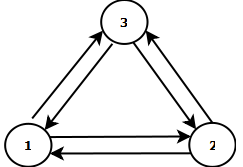
\includegraphics[scale=0.45]{final_images/Triangle.png}
%\end{center}
%	  \caption{Triangle network}
%	
%%\vspace{0.1in}
%\end{wrapfigure}
%
%\begin{figure}[htb]
%%\vspace{-0.3in}
% \begin{center}
%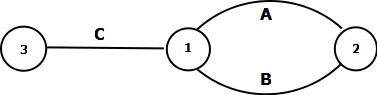
\includegraphics[scale=0.4]{final_images/Diagram3node.png}
%\end{center}
%	  \caption{Lasso network}
%	
%%\vspace{0.1in}
%\end{figure}

\begin{figure*}[tbh]
  \begin{center}
%    \subfigure[Mean download rate]{\label{fig:allisps_mean_throughputs}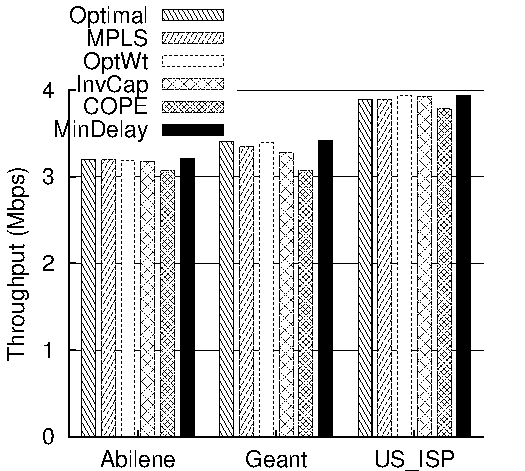
\includegraphics[width=35mm,height=30mm]{final_images/mean_throughput_hist_plot.pdf}}
    \subfigure[Triangle network]{\label{fig:triangle}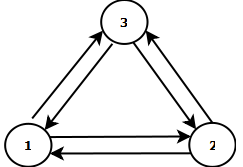
\includegraphics[scale=0.5]{final_images/Triangle.png}}
    \subfigure[Lasso network]{\label{fig:3node}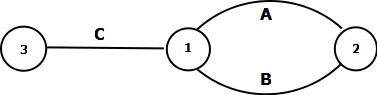
\includegraphics[scale=0.5]{final_images/Diagram3node.png}}
  \end{center} 
  \caption{Example networks}
\end{figure*}


%We explain it using the three node netowrk in Figure~\ref{fig:3node}.

%The objective of TE is to ensure the the link utilization in the network is at minimal level but location can alter its effects by changing the traffic matrix and hence the utilization of links in the network.


%\textbf{explain conditions}
The three-node network in Figure~\ref{fig:3node} exemplifies the above phenomenon. All links are assumed to have a capacity of 100 units and a constant delay. The top link A has a very small delay compared to the other two links that both have equal delay. Node 1 has 100 Mbps of demand that it can obtain from 2 as well as 3. In addition, there is 20 Mbps of demand at node 1 which it can obtain only from 2.  We assume that the aggregate demand at a node consists of a large number of user-initiated connections. When content can be downloaded from multiple locations, users initiate parallel TCP connections and the throughputs along paths in a parallel TCP connection are inversely proportional to the path delays. The TE scheme is assumed to be OSPF-based, i.e., shortest-path routing using configured link weights and traffic split equally among multiple paths with equal weights.

%\textbf{point: TE cannot be achieved since adaptation changes TM.}

Suppose the weights of the links A and B are unequal and the link A has more weight. As a result, all of the traffic between 1 and 2 is routed using only link B. 1 splits its demand of 100 Mbps using parallel TCP equally between links B and C. Thus, the traffic on links A, B, and C is  0, 70, and 50 respectively. In the next step, seeking to balance load better for this resultant matrix, the TE scheme sets both the links A and B to the same weight (hoping to achieve link utilizations of 35, 35, and 50 respectively).  Consider how parallel TCP connections respond to this change.
Assuming each TCP connection between 1--2 is pinned to only one of the two paths---as is commonly done in practice to achieve equal-cost multi-path (ECMP) splitting---50 Mbps of demand at 1 gets routed using parallel TCP connections over the link A and link C, and an equal amount using parallel TCP connections along the link B and link C. In addition, the 20 Mbps of background traffic is split equally among link A and link B as per ECMP.  Since link A has a much smaller delay than link C, the 50 Mbps of demand at 1 using parallel TCP along those two paths will flow entirely through link A. The remaining 50 Mbps using B and link C will get split equally across the two paths by parallel TCP. Thus, the traffic on the links A, B and C is 60, 35, and 25 respectively, which is different from what the TE scheme engineered for (namely, 35, 35, and 50). The resulting MLU of 0.6 is different compared to 0.5, the value that the TE scheme expected. 


%\textbf{explain conditions}
%The three-node network in Figure~\ref{fig:3node} exemplifies the above phenomenon. All links are assumed to have a capacity of 100 units and a constant delay. The top link 1--2 has a very small delay compared to the other two links that both have equal delay. Node 1 has 100 Mbps of demand that it can obtain from 2 as well as 3. In addition, there is 20 Mbps of demand at node 1 which it can obtain only from 2.  We assume that that the aggregate demand at a node consists of a large number of user-initiated connections. When content can be downloaded from multiple locations, users initiate parallel TCP connections and the throughputs along paths in a parallel TCP connection are inversely proportional to the path delays. The TE scheme is assumed to be OSPF-based, i.e., shortest-path routing using configured link weights and traffic split equally among multiple paths with equal weights.

%\textbf{point: TE cannot be achieved since adaptation changes TM.}

%Suppose the weights of the top and bottom links connecting 1 and 2 are unequal and the top link has more weight. As a result, all of the traffic between 1 and 2 is routed using only the bottom link. 1 splits its demand of 100 Mbps using parallel TCP equally between 1--2 (bottom) and 1--3. Thus, the traffic on links 1--2 (top), 1--2 (bottom), and 1--3 are  0, 70, and 50 respectively. In the next step, seeking to balance load better for this resultant matrix, the TE scheme sets both the top and bottom 1--2 links to the same weight (hoping to achieve link utilizations of 35, 35, and 50 respectively).  Consider how parallel TCP connections respond to this change.
%Assuming each TCP connection between 1--2 is pinned to only one of the two paths---as is commonly done in practice to achieve equal-cost multi-path (ECMP) splitting---50 Mbps of demand at 1 gets routed using parallel TCP connections over the bottom 1--2 link and 1--3, and an equal amount using parallel TCP connections along the top 1--2 link and 1--3. In addition, the 20 Mbps of background traffic is split equally among the two links between 1 and 2 as per ECMP.  Since 1--2 (top) has a much smaller delay than 1--3, the 50 Mbps of demand at 1 using parallel TCP along those two paths will flow entirely through 1--2 (top). The remaining 50 Mbps using 1--2 (bottom) and 1--3 will get split equally across the two paths by parallel TCP. Thus, the traffic on the links 1--2 (top), 1--2 (bottom), and 1--3 is 60, 35, and 25 respectively, which is different from what the TE scheme engineered for (namely, 35, 35, and 50). The resulting MLU of 0.6 is different compared to 0.5, the value that the TE scheme expected. 

%\tbd{
%We remark that the above examples assumed directed edges or multiple links between two nodes only for pedagogical simplicity. Straightforward extensions with neither assumption may be found in a technical report \cite{TR}.
%}

\subsection{Location diversity: Quantifying capacity}

How can we quantify the capacity achieved by a TE scheme in the presence of location diversity? In general, the capacity is a {\em region} that includes all of the traffic matrices that it can accommodate. However, quantifying the capacity of a TE scheme as a region may shed little light on its ability to tolerate typically encountered load spikes. Furthermore, it is cumbersome to compare TE schemes that achieve overlapping capacity regions. So, it is common to use a more concise metric such as the MLU to characterize the capacity with respect to a given traffic matrix. Intuitively, the inverse of the MLU serves as a metric of capacity, e.g., if a TE scheme achieves an MLU of 0.25 for a given matrix, then it can tolerate up to a 4$\times$ surge in the load represented by the matrix. Unfortunately, as the example in Figure \ref{fig:3node} shows, MLU is not a meaningful metric of capacity when application adaptation to location diversity  determines the traffic matrix.  

With location diversity, the demand is best represented as a ``content matrix'' that specifies for each node and each content the traffic for that content at that node and the set of source locations from where that content can be downloaded (e.g., 100 Mbps at node 1 downloadable from 2 and 3, and 20 Mbps at node 1 downloadable from node 2, in Figure \ref{fig:3node}). The traffic matrix corresponding to this demand depends upon the underlying routes and application behavior (e.g., how parallel TCP splits traffic across the download locations). Furthermore, scaling the demand does not simply scale the traffic matrix entries by the same factor. In general, it is difficult to predict how application behavior might change the traffic matrix for a projected surge in demand, as that change depends upon the underlying routes that in turn depend upon the original traffic matrix. Indeed, as the example shows, even if the demand is unchanged, the mere act of engineering routes can change the traffic matrix yielding a different MLU than expected.


%To appreciate this point, consider the example shown in Figure \ref{fig:mlu_toy}. Node 1 has a demand of 100 Mbps for content that can be fetched from either of nodes 2 or 3. Suppose node 1 splits the demand equally between the two locations, thereby resulting in an MLU of 1 by saturating the left link. Note that all TE schemes will result in the same routing as there is at most one route between each pair of nodes. Now suppose the demand at node 1 doubles to 200 Mbps. Node 1 can still satisfy its demand by fetching 50 Mbps and 150 Mbps along the left and right links respectively. Note that the MLU remains unchanged at 1 even though the demand has doubled. Furthermore, the doubling of demand does not simply scale the traffic matrix entries linearly, but instead changes them based on application behavior (e.g., based on how parallel TCP splits traffic across the two download locations). In general, it is difficult to predict how application behavior might change the traffic matrix as demand increases, as that change depends upon the underlying routing that in turn depends upon the original matrix. Indeed, even if the demand remains unchanged, the mere act of engineering routes (not observable in Figure \ref{fig:mlu_toy} as there is no route diversity) can change the traffic matrix when applications have location diversity.

%It is difficult to predict \CAP{} using MLU if the network has application adaptation. This is because application adaptation can change the traffic matrix.  We show it using an example.  In Figure~\ref{fig:load-1} at load = 1.0 User node has a demand for 100Mbps traffic and it splits its demand equally and downloads 50Mbps each from N1 and N2. In Figure~\ref{fig:load-2}) at load = 2.0, the User node can still serve its demand by downloading 50Mbps from N1 and 150Mbps from N2. The metric MLU is not relevant in both cases since the application can change the traffic matrix to serve its demand. Empirically too we observed that the MLU value did not show a clear demarcation at a load where network is below capacity and the load where network is above capacity.

\subsubsection{An empirical capacity measure}
\label{sec:SPFdefinition}
%\textbf{proposing a new metric}

We propose a new metric, {\em surge protection factor} (SPF), to quantify the capacity achieved by a TE scheme with respect to a traffic matrix. Let $E$ denote a TE scheme, $M$ the demand specified as a content matrix. When there is no location diversity, $M$ can be easily transformed to a unique traffic matrix $T(M)$. Let  MLU$(E,T(M))$ denote the MLU achieved by $E$ given the traffic matrix $T(M)$. In this case, SPF$(E,M)$ is simply the inverse of MLU$(E,T(M))$, i.e., the factor of increase in the demand that can be satisfied. However, in the case when there is location diversity, SPF$(E,M)$ is an {\em empirical} measure of the satisfiable increase in demand computed as follows. Let $kM$ denote the demand that scales each entry in $M$ by a factor $k>1$. Then, SPF$(E,M)$ is defined as the largest $k$ such that the routing computed by $E$ (for the matrix $T(M)$) can satisfy the demand $kM$.

Determining if an engineering scheme can satisfy a projected demand is difficult as it requires us to accurately model application adaptation to location diversity, so SPF is useful mainly as an empirically measured capacity metric. To this end, we describe our experimental setup next.
